\section{Aperture Photometry}
\label{sec:aperture_phot}
In order to determine the flux of different objects in astrophysics, like stars and planets, aperture photometry can be used. This method sums the counts of the pixels inside a certain aperture around the star. In our case this aperture is usually a circle. In order to account for the background noise an annulus around the aperture is taken and the mean of the summed up pixels inside the annulus is subtracted from the apertures pixels. The flux of this aperture is then given by \cite{Gisin}
\begin{equation}
	F_{ap} = F_{tot} - n_{px} \langle F_{bg} \rangle ,
\end{equation}
where $F_{tot}$ is the total flux inside the aperture (sum up the pixel values inside the aperture), $n_{px}$ is the number of pixels inside the aperture and $\langle F_{bg} \rangle$ is the mean background per pixel. This mean background per pixel is defined through the annulus and calculated from
\begin{equation}
	\langle F_{bg} \rangle = \frac{1}{m} \sum_{i=1}^{m} c_{i} ,
\end{equation}
where $m$ is the number of pixels in the annulus and $c_{i}$ the respective pixel value.
Figure \ref{fig:aperture_ex} shows an example for a possible aperture and an annulus around a star, which can be used to do an aperture photometry.
\begin{figure}[H]
	\centering
		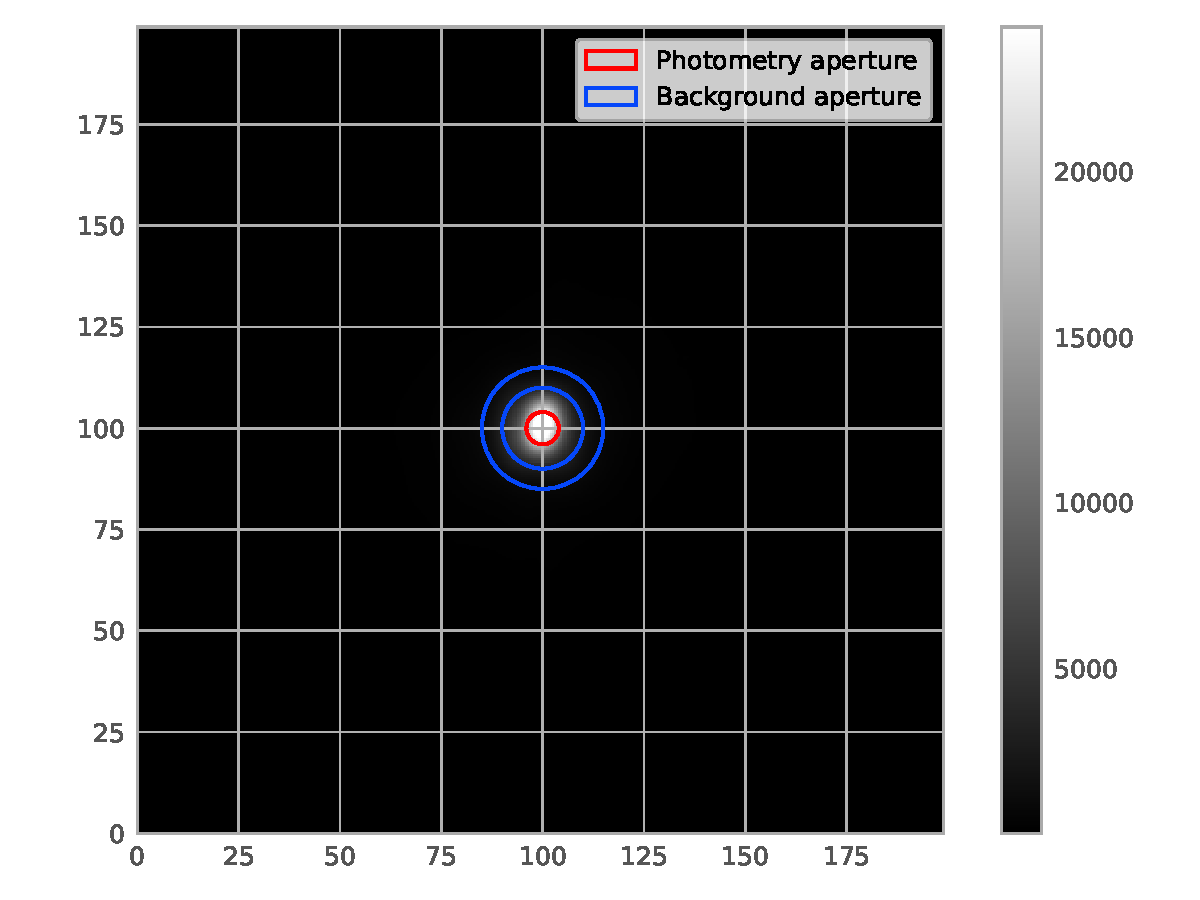
\includegraphics[width=0.9\textwidth]{pics/aperture_example.pdf}
		\caption{An aperture photometry for the star in the center, where the red circle indicates the aperture used and the two blue circles define the annulus used for the background subtraction.}
		\label{fig:aperture_ex}
\end{figure}
We choose the radius of the aperture to be 6 pixels. From the figure one can see that we chose the annulus not directly after the aperture, but this is just one way to do it. One could also choose the annulus directly after the aperture or choose a different distance between the annulus and the aperture. However the annulus should give a good approximation for the background inside the aperture and therefore it should not be too far away from the aperture. We choose a small distance of 4 pixels between the aperture and the annulus, because we want that as little starlight (in this case) as possible is included in the annulus. If we plot the counts per pixels which are included in a certain radius around the star, as it is done in figure \ref{fig:annulus_radi} we see that after around 10 pixels the increase is decreasing rapidly. That is where there is only little starlight left. This is why we choose the annulus to go from a radius of 10 to 15 pixels. 
\begin{figure}[H]
	\centering
		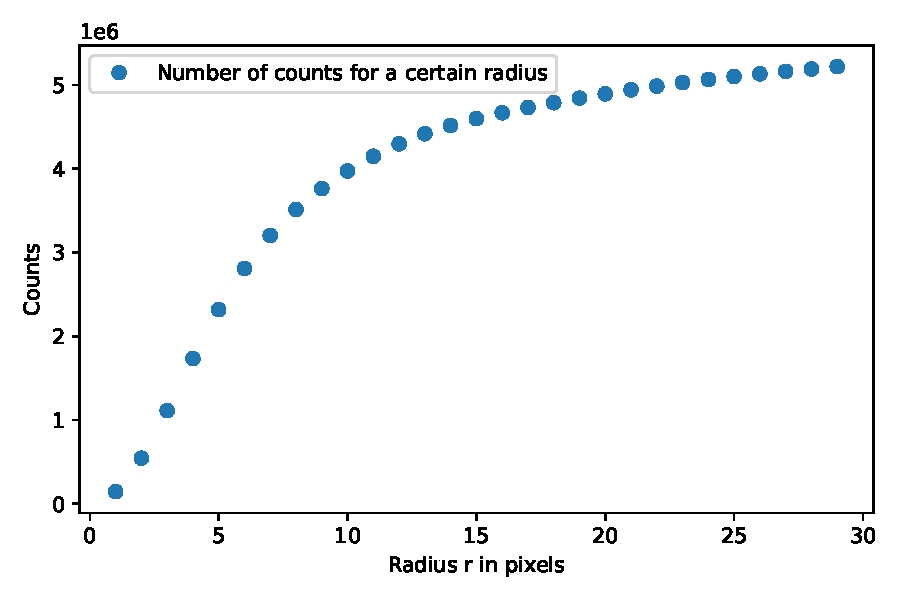
\includegraphics[width=0.8\textwidth]{pics/CountsPerRadius.pdf}
		\caption{The total flux of the star is calculated for different aperture radii and plotted. This shows that after a radius of 10 pixels the contribution from the star is almost gone.}
		\label{fig:annulus_radi}
\end{figure}

\subsection{Aperture photometry and ghosts}
In order to detect exoplanets one can use aperture photometry. In this subsection we are going to do these steps for the two ghosts which we have in our data from the circumstellar disk HD142527, in order to demonstrate how this could be done for an exoplanet and to learn more about ghosts.\\
A ghost is a copy of the star, which is created by the back-reflection of the star on optical components of the telescope. Figure \ref{fig:ghosts} is an image of HD142527, where the two ghosts are indicated. We see that the ghost on the top right (we will call it ghost 1) is brighter than the ghost on the bottom left (ghost 2). 
\begin{figure}[H]
	\centering
		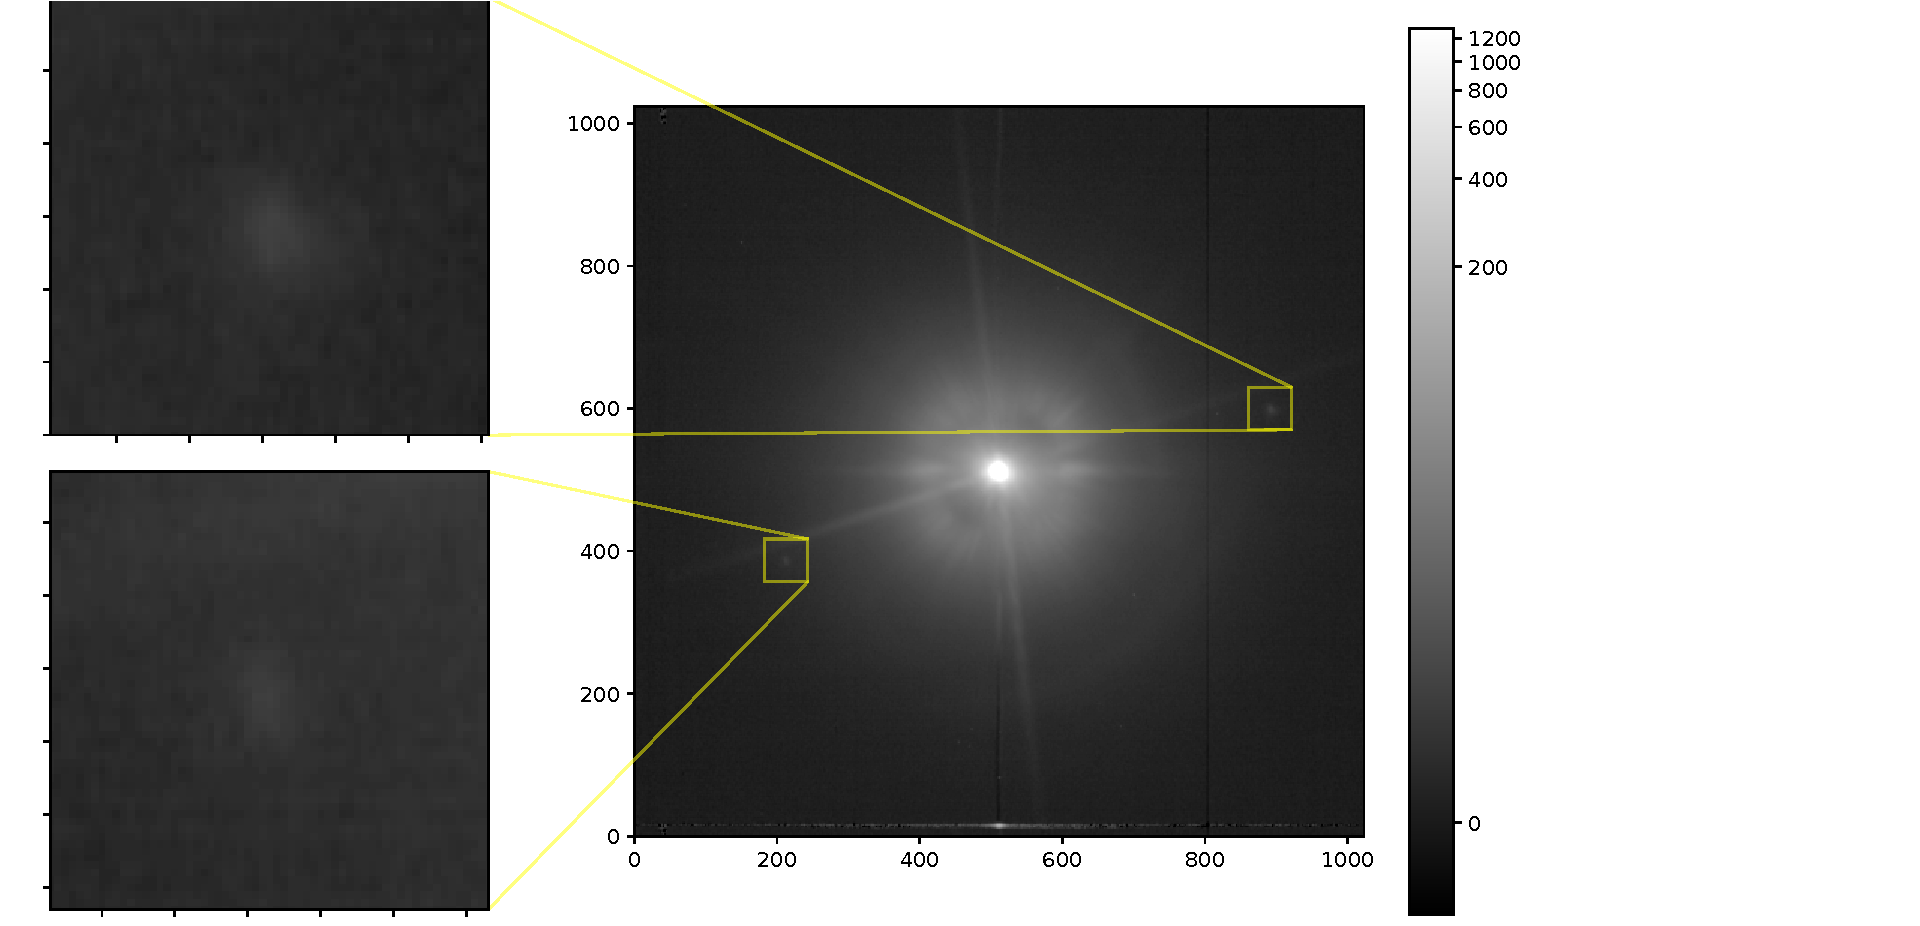
\includegraphics[width=1.3\textwidth]{pics/Ghosts.pdf}
		\caption{An image of the circumstellar disk HD142527, where the two ghosts are indicated.}
		\label{fig:ghosts}
\end{figure}
If we want to confirm the signal from our ghost or also from other objects like exoplanets, which usually can not be seen by eye, we use the signal to noise ratio $S/N$. This means we do aperture photometry for several points around the star which are at the same separation from our star as the ghost (or exoplanet etc.), as shown in figure \ref{fig:ap_phot_gh1}. From these aperture fluxes we can calculate the standard deviation $\sigma$ and the signal to noise ratio. If the signal to noise ration is larger than $3 \sigma$, this means that we have a source (ghost, exoplanet) at this position. 
\begin{figure}[H]
	\centering
		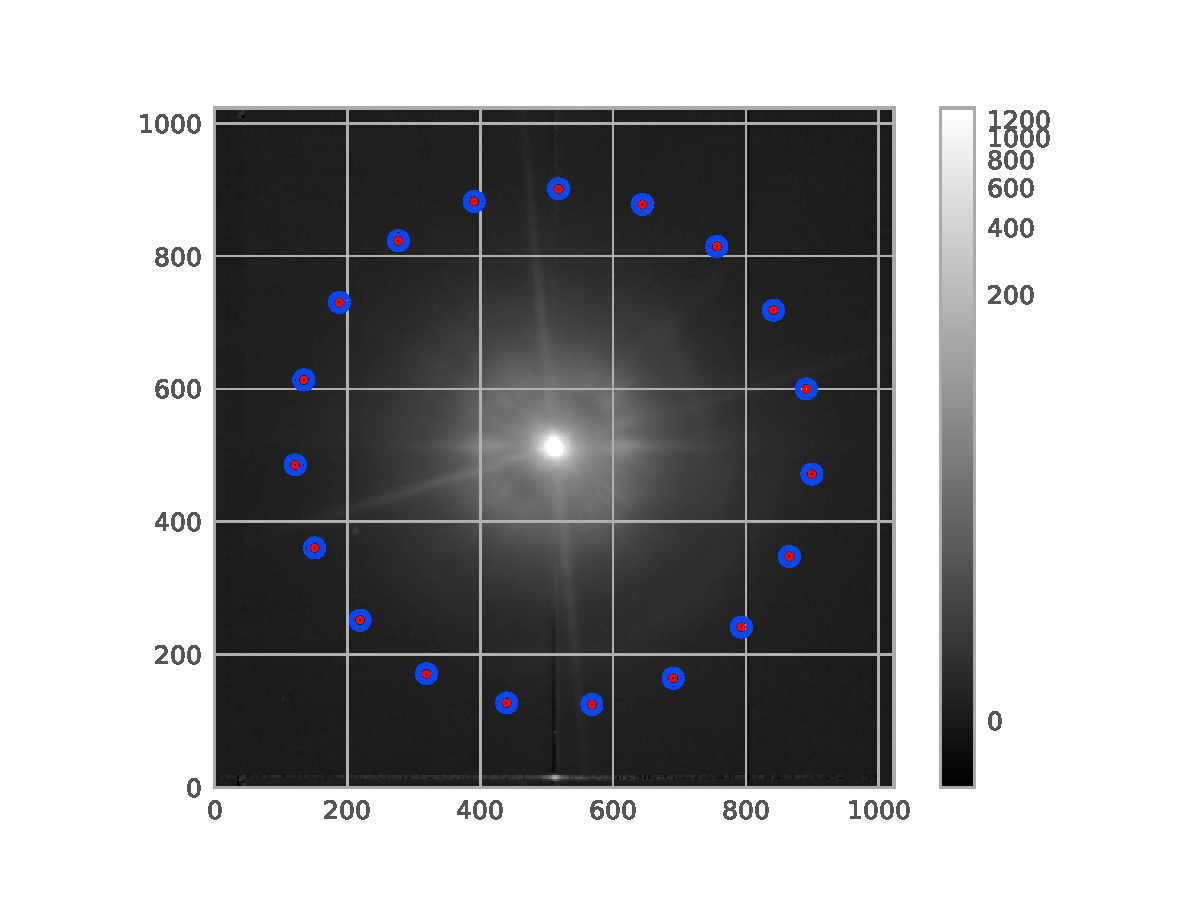
\includegraphics[width=0.9\textwidth]{pics/aperture_photometry_19_ghost1.pdf}
		\caption{In order to confirm the signal from the ghost, we do aperture photometry for several points around the star which are at the same distance from the star as the ghost. We then calculate the standard deviation of all the aperture fluxes and from there find the signal to noise of the ghost's aperture. If the signal to noise is larger than the standard deviation, the position of the ghost is confirmed.}
		\label{fig:ap_phot_gh1}
\end{figure}
The standard deviation is calculated by
\begin{equation}
	\sigma = \sqrt{\frac{1}{k-2} \sum_{ap=2}^{k} (F_{ap} - F_{mean})^2} ,
\end{equation}
where the aperture of the ghost is at $ap=1$, $k$ is the total number of apertures and $F_{mean}$ is the mean flux of the apertures (without the aperture flux of the ghost) given by
\begin{equation}
	F_{mean} = \frac{\sum_{ap=2}^{k} F_{ap}}{k-1} .
\end{equation}
From this we can find the signal to noise ratio as
\begin{equation}
	S/N = \frac{F_1 - F_{mean}}{\sigma} .
\end{equation}
The results we get from our data about the ghosts are shown in table \ref{table:ghosts}. It confirms that ghost 1 is where we expected it to be, since its signal to noise is larger than $3 \sigma$. For ghost 2 this is not the case. The signal to noise is larger than the standard deviation, which tells us that there might be an object, but the confidence interval is only $2 \sigma$. This is not enough to confirm the detection. \\
We also want to compare the intensity of the ghosts to the intensity of the star. For this we calculate the ratio between the aperture flux of the ghost and the star. We find that the ghosts are about $10^{-4}$ times less bright then the star. 
\begin{table}[H] 
\centering
\begin{tabular}{|c|c|c|}
\hline
 & \textbf{Ghost 1} & \textbf{Ghost 2}\\
\hline
$\mathbf{S/N}$ & $33.9$ & $16.5$\\
\hline
$\mathbf{\sigma}$ & $7.9$ & $9.8$\\ 
\hline
\textbf{Ratio} & $11.5 \pm 0.4 \cdot 10^{-5}$ & $6.7 \pm 0.5 \cdot 10^{-5}$\\
\hline
\end{tabular}
\caption{Signal to Noise of the ghosts and their brightness with respect to the star. The standard deviation $\sigma$ is given in counts.}
\label{table:ghosts}
\end{table}
